\documentclass[11pt,a4paper]{article}
\usepackage[T1]{fontenc}\usepackage{lmodern}
\usepackage[margin=22mm,headheight=14pt]{geometry}
\usepackage{amsmath,amssymb,bm,booktabs,tabularx,array,graphicx,float,fancyhdr,microtype,xcolor}
\usepackage[colorlinks=true,linkcolor=blue!45!black,urlcolor=blue!45!black,citecolor=blue!45!black]{hyperref}
\setlength{\parindent}{0pt}\setlength{\parskip}{5pt}\renewcommand{\arraystretch}{1.15}
\pagestyle{fancy}\fancyhf{}\fancyhead[L]{\small QFT Project B | Step 5}\fancyhead[R]{\small Group B}\fancyfoot[C]{\thepage}
\newcommand{\dd}{\mathrm{d}}
\begin{document}\hypersetup{pageanchor=false}
\begin{titlepage}\centering\vspace*{3mm}

\includegraphics[width=36mm]{assets/bits_logo.png}\par\vspace{13mm}
{\Large\bfseries BITS PILANI K.K. BIRLA GOA CAMPUS\par}\vspace{3mm}
{\large\bfseries Department of Physics\par}\vspace{18mm}
{\LARGE\bfseries What Quantum Trace Can\\[2mm] a Heavy Particle Leave?\par}\vspace{6mm}
{\large Curvature--Spectator Entanglement\\and the Cosmological Collider\par}\vspace{10mm}
{\large\bfseries Step 5: Gaussian Entanglement\par}\vspace{17mm}
{\Large\bfseries Group-B\par}\vspace{5mm}
\begin{tabular}{ll}Priyansh Rawat & 2023B5A70968G\\Mayank Sinha & 2023B5A70942G\\Samarth Bhatnagar & 2023B5A70853G\end{tabular}
\vfill{\large Under Professor: Rudranil Basu\par}\vspace{7mm}{29 October 2026\par}
\end{titlepage}\setcounter{page}{1}\hypersetup{pageanchor=true}
\section{Covariance, entropy and the reliability window}
For one real sector, $V=\operatorname{Re}(\mathcal M\mathcal M^\dagger)$ and $V_q$ is its light-field $2\times2$ block. The reduced symplectic eigenvalue is $\nu_q=\sqrt{\det V_q}$ and $S_q=s(\nu_q)$. The two full-state symplectic eigenvalues must remain $1/2$ because quadratic evolution preserves the purity of the initial state.
Outside the horizon, large correlated entries can make the determinant ill conditioned. We first apply the local canonical shear $\widetilde\Pi_q=\Pi_q+Q/x$, which leaves $\det V_q$ invariant. Covariance products use extended-precision arithmetic; a local canonical scaling balances the matrix before evaluating its full symplectic eigenvalues.
We accept samples with commutator residual $<10^{-6}$ and full-state eigenvalue error $<10^{-5}$. The history is shown only up to the first failure of these criteria. For the benchmark, the last sample in this contiguous reliable interval is $x=5.492\times10^{-4}$. The evolution is not extrapolated past it.
\begin{figure}[H]\centering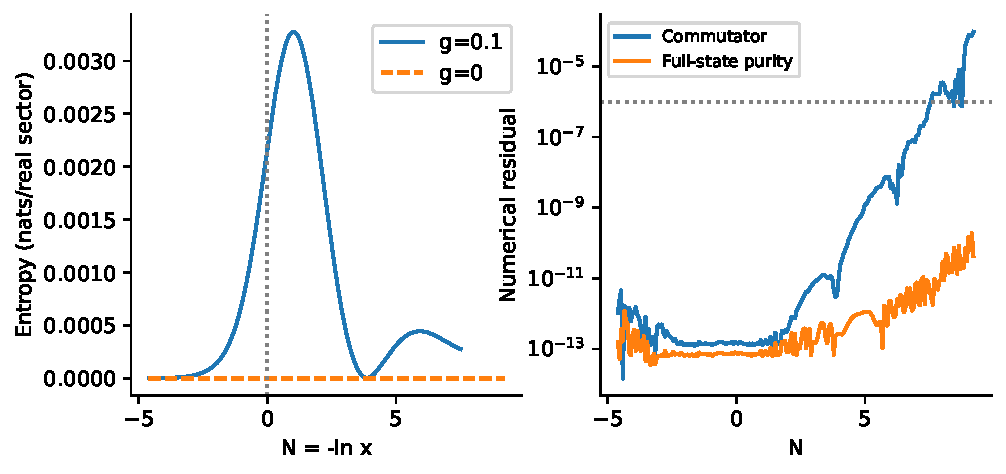
\includegraphics[width=.91\linewidth]{figures/entropy_and_purity.pdf}\caption{Benchmark entropy and numerical diagnostics. Horizon exit is $N=0$. The zero-mixing curve measures the numerical floor; it is not physical inter-field entropy.}\end{figure}
\newpage
\section{Mass/mixing scan and physical interpretation}
We compare $M=1.6,1.8,2.0,2.4$ and $g=0,0.05,0.1,0.2$ at the same $x=1,0.1,0.01,0.001$. All 64 requested comparison rows pass the stated diagnostics. Entropy is quoted per real sector; a generic nonzero momentum pair has twice this value.
At $M=2$, $g=0.1$, $x=0.01$, we obtain $S_q=1.846\times10^{-4}$ nats and a fractional light-power increase of $0.003714$. Reversing $g$ changes the entropy by $6.003\times10^{-12}$. This checks the $\sigma\mapsto-\sigma$ symmetry. The largest zero-mixing entropy in the sampled history is $2.227\times10^{-9}$, which sets a numerical floor rather than an entanglement detection.
\begin{figure}[H]\centering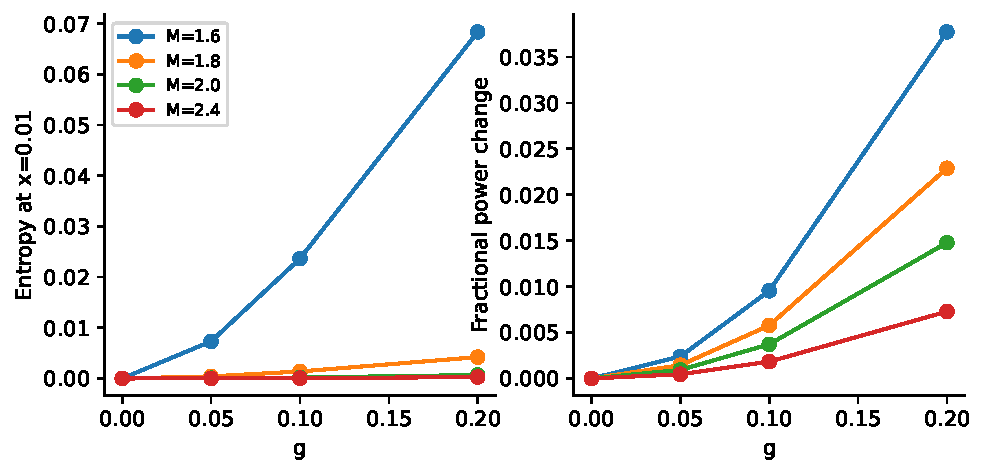
\includegraphics[width=.91\linewidth]{figures/mass_mixing_scan.pdf}\caption{Entropy and fractional power change at the common time $x=0.01$. They measure different aspects of the Gaussian state.}\end{figure}The time history is not assumed monotone: exchange of correlations can produce growth and decrease while the full state stays pure. These Gaussian entropies omit cubic-interaction corrections and will be compared with a leading cubic bispectrum.\begin{thebibliography}{9}\small
\bibitem{gaussian} C. Weedbrook et al., \emph{Gaussian Quantum Information}, Rev. Mod. Phys. 84, 621 (2012), \href{https://arxiv.org/abs/1110.3234}{arXiv:1110.3234}.\end{thebibliography}
\textbf{Code and supporting data:} \href{https://github.com/rawatpriyansh17/QFT-PROJECT-GROUP-B/tree/main/step5}{step5 on GitHub}.\newpage\section*{Contributions (equal)}\begin{center}\begin{tabularx}{\linewidth}{p{33mm}X}\toprule Member & Contribution\\\midrule Priyansh Rawat & Covariance and entropy derivation; interpretation.\\[3mm]Samarth Bhatnagar & Purity, zero-mixing and sign-symmetry validation.\\[3mm]Mayank Sinha & Mass/mixing scan, reliability mask and figures.\\\bottomrule\end{tabularx}\end{center}\end{document}